\cleardoublepage
\counterwithout{figure}{section}
\counterwithout{table}{section} 
\counterwithout{equation}{section}
\counterwithin{figure}{chapter}
\counterwithin{table}{chapter} 
\counterwithin{equation}{chapter}


\chapter{Assignment}
\label{sec:aufgabenstellung}
 In frame of this thesis a process is to be developed for generation of the dental color shades using an inkjet printer.  The mechanic aspects of responsible for the movement are not included to the project. A stepper motor driven system responsible for the coordinated movement of the axes controlled by a SmoothieBoard v2-mini is provided by the project partner Bredent GmbH. The specifications of the printing system, like a single drop volume or the max printing distance and angle are to be determined. 
 
 Afterwards, an adequate droplet generator is to be selected. The diameter of the nozzle is as important as the driver technology generating the droplets, which has a direct effect on the optical resolution of the printed pattern. With piezoelectric droplet generators, smaller and faster drops are possible but electromagnetic ones are cheaper. The quantitative coloring behavior depending on the absorption characteristics of the dental ceramic is an unknown to the state of the research and the technology. The shades of the dental colors are to be brought about using the main colors with the highest saturation level and a brightener, which is a water based diluter with  an identical composition to the inks, except lacking the metal-ionic coloring agent. The proportions of the ink and the diluter is not the only parameter affecting the shade of the generated color, but also the application sequence can have a significant effect on the optical perception. Since the translucency of the dental zirconia effects the level of color reflection, the depth of the colored section can have an undeniable effect on the natural look of the dental crown. 
 
 At last, the generated shades are to be verified with the existing color standards. The receipt for each single shade generation has to be prepared. The deployed droplets are not expected to fly and settle on the contact point drying on the surface, but are expected to be absorbed and spread inside the porous material. This nature of the interaction between the ink in its fluid form and porous zirconia defines the system as a nonlinear three dimensional fluid dynamics problem. A model is to be generated taking the every compensational aspect of the nonlinear ink behavior, in order to achieve a point accurate color acquisition.
 
 

\chapter{Expected Advantages and Functions of the Solution}
One of the most important advantages is quantification of the coloring process followed by the printing process. Until this day, the crown coloring process is made by dental technologists all around the world. In other words, all of the dental replacements are partially handcrafted. In the market, hand crafted is another word for made by a craftsman, specifically for the unique owner of the product. Just as any other product on the market, the word handcrafted has a prominent effect on the price tag of the item. The word handcrafted also means the product has some tiny error, a nuance special for each unique sample. If the object of interest is a decor for the home of the consumer, it is one of the most welcome properties. However, if the object of interest is an implant, which is to be carried all the time on the comsumer's body as a part of the it, the property everyone is looking for is perfection. A perfect shape, color, consistency and harmony is a standard to evaluate the quality of the work done by the dentist and of course involving the dental technologist. The quantification of the coloring process is the most important advantage of the solution when it is considered looking from this aspect. Thus, the error can be terminated and the quality deviation can be limited to an acceptable variance. 

Another aspect to consider is the ink costs. Each of the ink bottles are labeled with the same price tag by the manufacturer. However, not all of the ink bottles contain a material worth the same value actually. The shades of the colors ranging from 1 to 3.5 are only diluted versions of the bottle with the shade 4.0. Buying the most concentrated tone and diluting it is here an economical solution, as it is in every other section of the industry. Also, the whole spectrum of shades can be obtained with only 4 ink bottles and a brightener by halftone printing. The required purchase variety, transportation costs, and the space requirement are all reduced with the usage of only the most saturated shades.

\chapter{Solution Structure}
The structural concept is based on the utilization of a 5-axis printing system. A basic microcontroller designed for the automation of the router systems is connected to stepper motors and encoders to control the coordinated printing processes. 4 base colors with the highest saturation levels (A, B, C and D4) are to be used with the brightener to color the dental zirconia, instead of 17 bottles consisting of 16 predefined shades plus the brightener. The amount of the brightener defines the shade of the color. Therefore, the space requirement of the machine is reduced. The inks and the brightener are continuously fed into a rotary distribution valve and are in their neutral status not flowing in any direction. As soon as the rotary valve opens the gate of any incoming pipe,the flow is permitted to the droplet ejector.  

\bigskip

\begin{figure}[H]
	\centering
	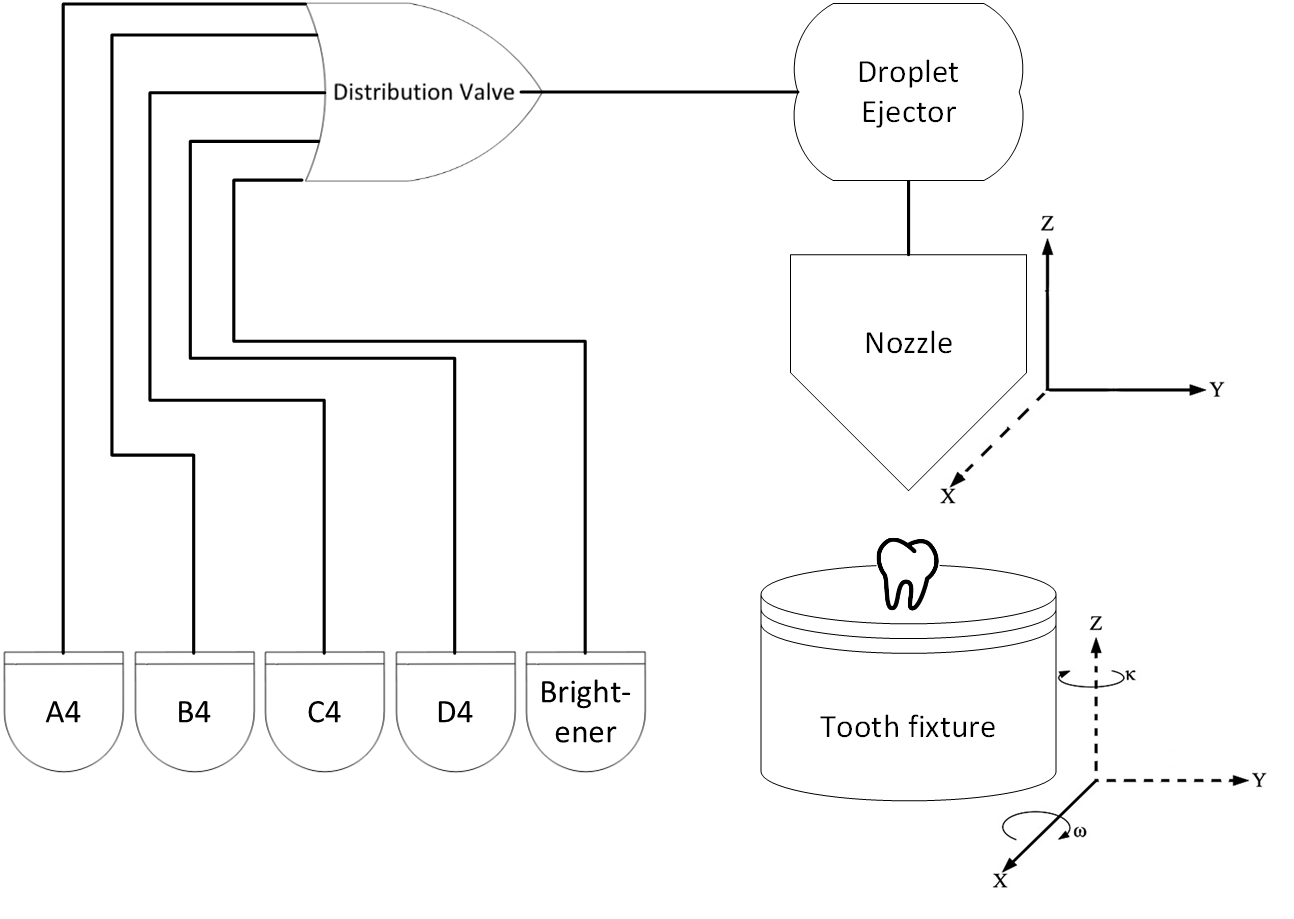
\includegraphics[width=0.9\textwidth]{grafiken/SolutionStructure.jpg}
	\caption{Solution Structure}
	\label{fig:SolutionStructure}
\end{figure} 

\bigskip

A serial communication between the controller and the rotary valve arranges the position of the rotary valve and the duration to hold on in that position. The required mixture is dosed and pulled by the droplet ejector and deployed through the nozzle, driven by the pressure difference between the ink bottles at the beginning of the cycle and the atmosphere. A 3-axis table and the 2-axis nozzle holder are responsible for the coordination of the flying drops and the point on the surface of the dental crown where the drops need to land during the printing process.

\chapter{Solution Processes}
\label{sec:Lösungsprozesse}
The process concept is realized in three stages. Each stage depends on the previous one and cannot be proceeded to, before the previous one is completed.

\bigskip

\begin{figure}[H]
	\centering
	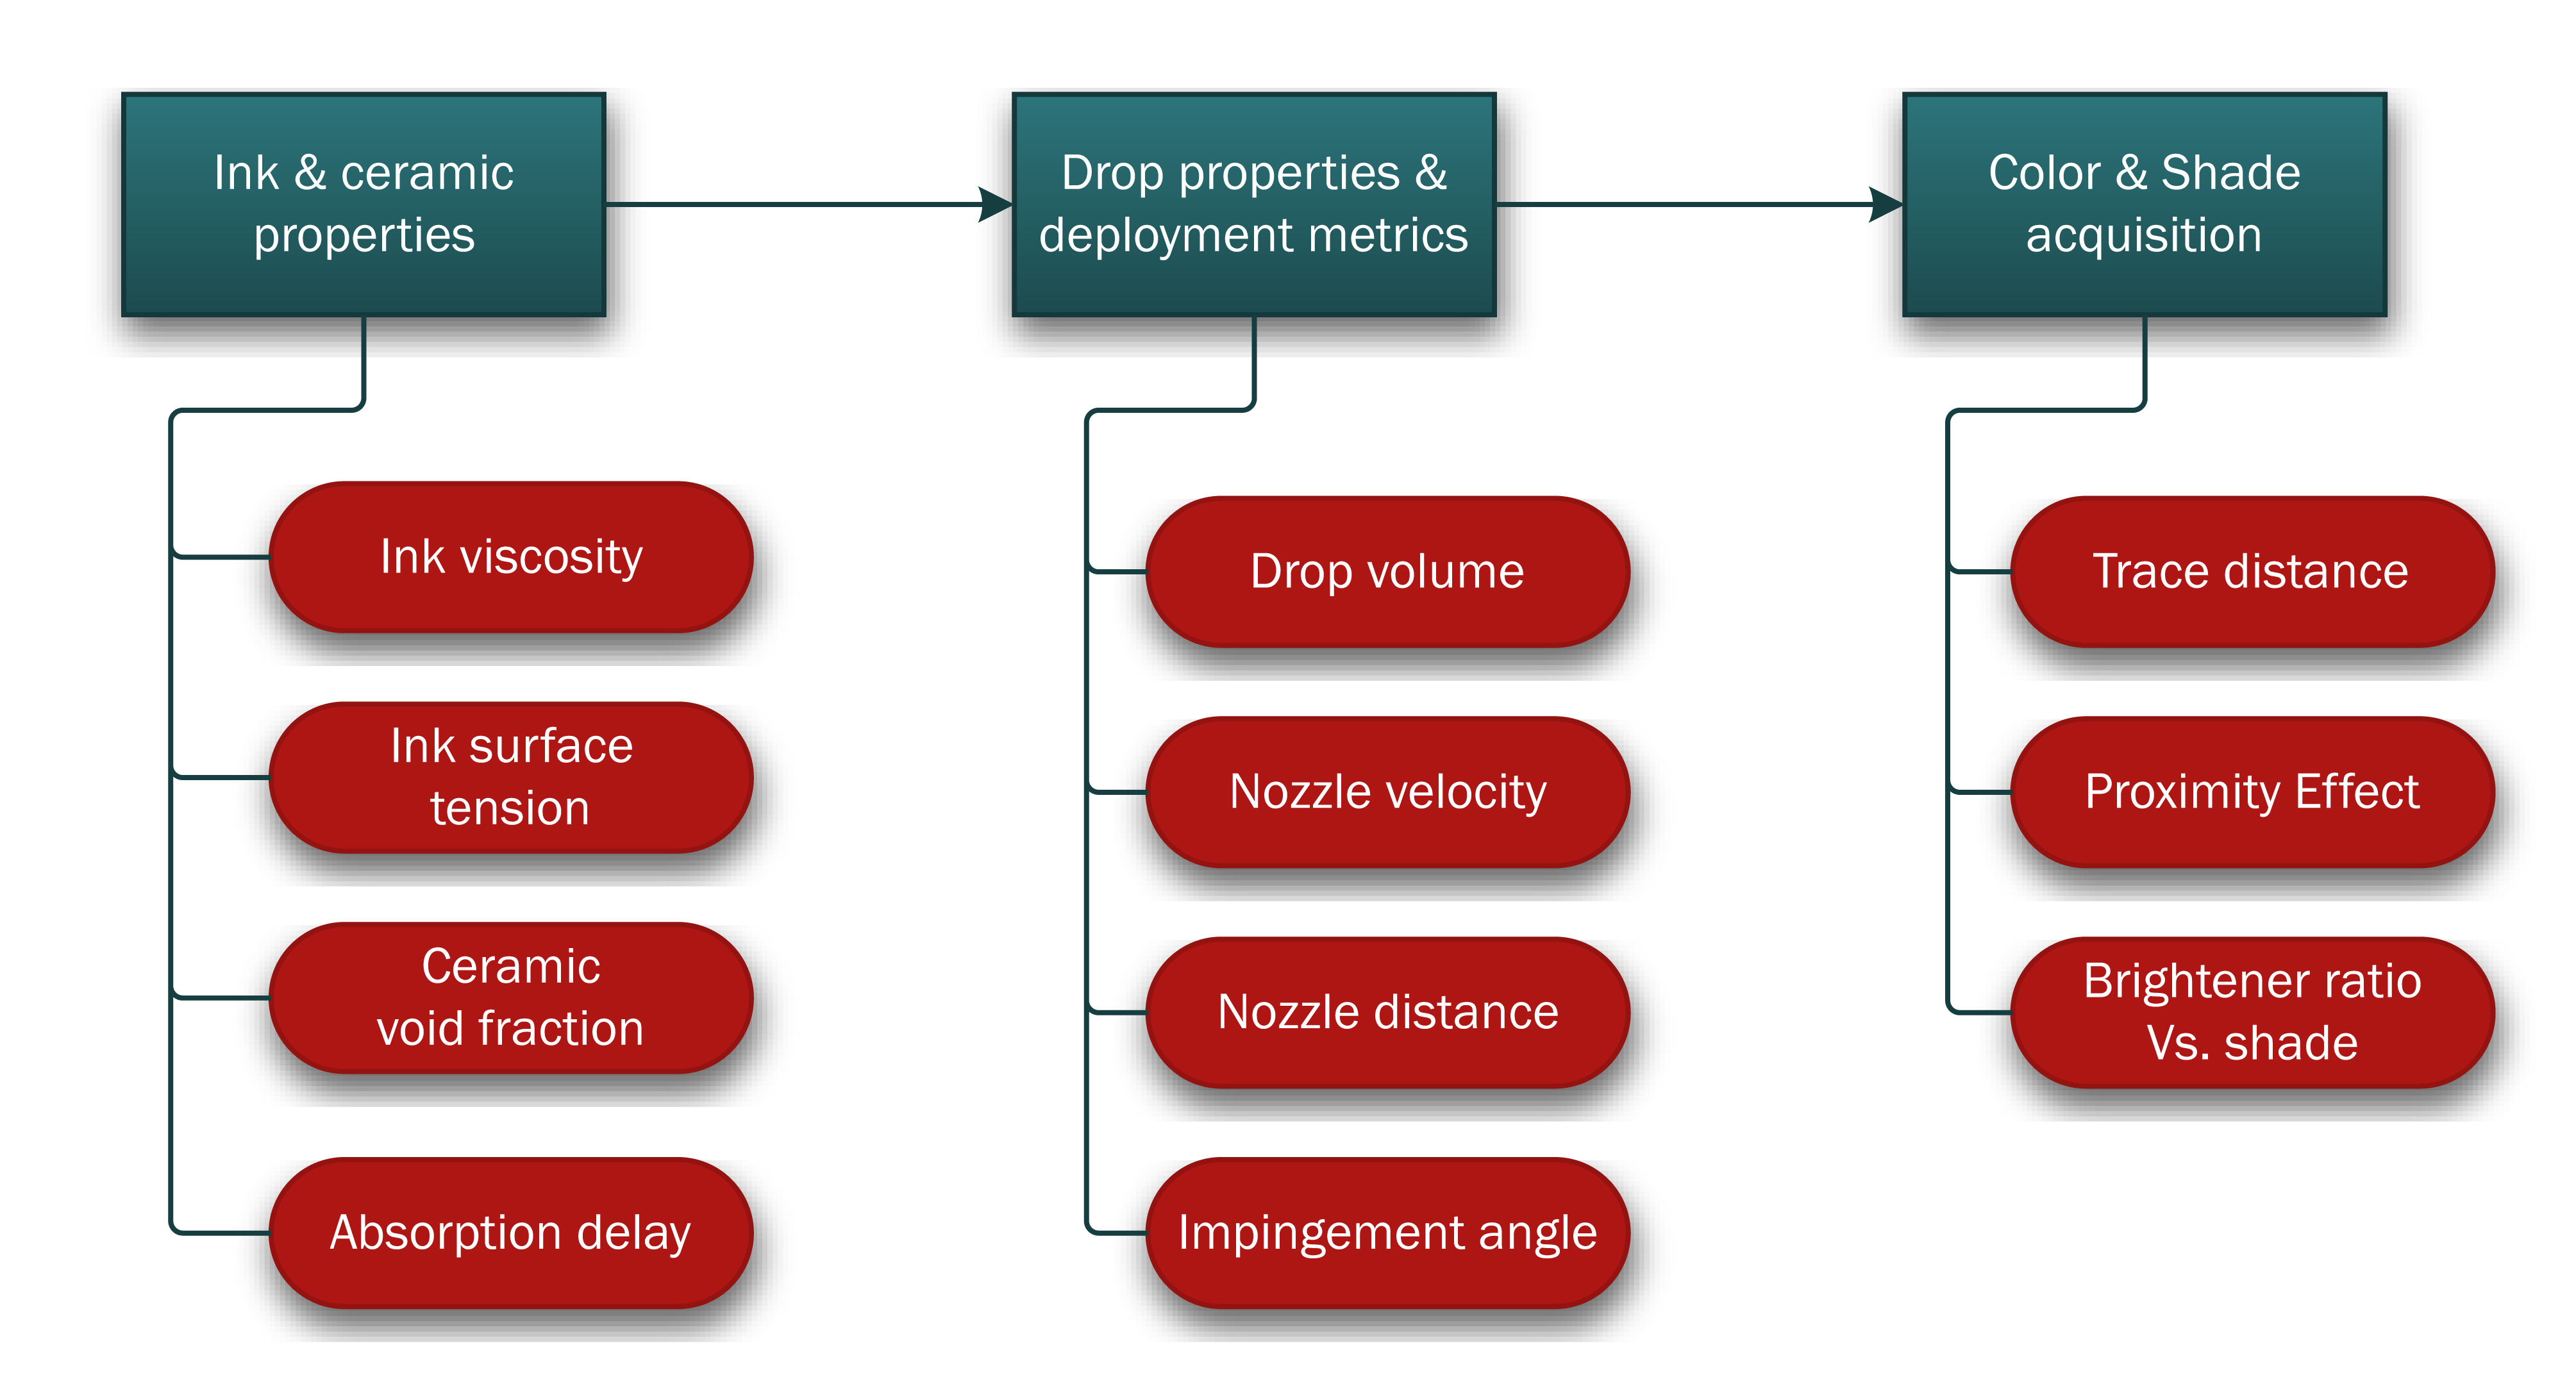
\includegraphics[width=0.9\textwidth]{grafiken/SolutionProcesses.jpg}
	\caption{Solution Processes}
	\label{fig:SolutionProcesses}
\end{figure} 

\bigskip


 First stage is finding the ink and ceramic properties, such as ink viscosity and surface tension, ceramic void fraction and ink absorption time. Depending on these experimentally acquired parameters the equations \ref{eq:InfTime} and \ref{eq:SpreadingDia} can be utilized  in the progress of the model generation for the drop deployment algorithm for an arbitrary pattern to be printed on the zirconia material. 
 
 Second stage is planned to help determine the parameters defining the printing system. It basically focuses on the settlement of drop properties and deployment metrics, which consist of drop volume, nozzle escape velocity of the drops, the optimal distance between the nozzle and zirconia surface and the angle between the drop projectile and the surface. The drop volume has to be determined as soon as possible, because it directly affects the selection of the actuator which is to be used as the drop ejector. Selection of a larger drop size means a shorter printing time. However it also means that the resolution is supposed to become lower. Due to the absorption characteristics of the zirconia material, a critical drop size is expected to cause a significant effect on the diameter of a painted spot. In other words, deploying the same amount of ink on the same spot using drops with a volume of smaller than 5 nL could give the same printed spot diameter.In comparison to the aforementioned drop volumes, using  10 or 20 nL drops to apply the same amount of ink on a single point could result with an unexpectedly larger spot size with lower central intensity. This critical drop size has to be determined, in order to proceed to the rest of the experiments.  
 
 The projectile velocity of the drops is one of the most important parameters affecting the printing system on a temporal basis and also the spreading characteristics of the ink within the porous medium. It is known that for Weber numbers higher than 50, the drops are expected to splash upon the impact with the surface \citep{clarke2002spreading}.
 
 \bigskip
 
 \begin{equation}\label{eq:weber}
 We=\frac{\rho rv^2}{\gamma}
 \end{equation}
 
 \bigskip
 
 The maximum distance of the nozzle to the zirconia surface has to be limited. The projectile of the droplets are not perfectly identical. There is a deviation of the impact point, because of the factors like a slight change of the nozzle escape angle of an arbitrary droplet or drag caused by the spontaneous fluctuation of the air flow inside the printing chamber. The longer the fly distance of the droplets are, the less accurately they will meet the same point. So the deployment distance for the droplets should be as short as possible. However on the other side the geometry of the crown creates the second boundary of the problematic. The concave structures on the upper side of the teeth carrying out the chewing function pose a collision danger with the nozzle. This is a situation where the printing angle is also influential. 
 
 The aspects to be considered under the third stage are employed to conduct an experimental approach to color and shade acquisition. In order to arrive there some parameters have to be determined. Firstly the appropriate trace distance for the selected drop size is to be concluded, depending on the experiment with varying trace distances, which is the distance between two sequential lines on the printed surface. The proximity effect is the second nonlinear parameter affecting the print resolution and color distribution, which refers to how the proximity of two colored areas affect the shade of the uncolored area in between.Finally the dependency of the shade on the brightener ratio is to be determined. For a liquid inside a bottle it is very easy to come to a final conclusion. However, the porous translucent medium has a huge influence on the perceived shade, because of the  reflections form various depths of the material and photons following diverse paths through the sintered zirconia to the eye of the observer.
 
 All of the aforementioned tasks are to be carried out so at the end a model can be generated. This model has to work as an algorithm to calculate the input pattern for a desired arbitrary shade map of a dental crown geometry. The coloring behavior on the printed sample has to be compared with the virtually printed geometrical model.
 

\chapter{Distinctive Features of the Solution}
\label{sec:Unterscheidungsmerkmale}
The most contemporary dental laboratory of today still has to do the coloring process manually. A dental technologist uses brushes to apply tens of bottles of ink shades to the dental crowns one by one following the procedures described by dental zirconia ink manufacturers. Coloring each tooth takes about 5 minutes and about 100 precise brush strokes. This is a process which requires a high patience and repeatability. This project is the first automated printing approach in dental coloring sector. With the automation of the procedure many advantages are expected. The accuracy of shade acquisition is to be guaranteed because of the quantified and digitalized coloring procedure. The variation between the sequential teeth are to be minimized. Shorter lead times can be realized upon the optimization of the printing method, which is to be accompanied by lower costs due to the automation and shortened process time.

Another novelty of the project is the discontinuation of the requirement for a bottle for every single shade of each color. The lighter shade of each color are only bottle mixtures of the brightening fluid and the darkest shade of that color by the manufacturer. The mixtures do not posses a linear ratio for the contained ink and brightener depending on the color shade. The mixture is prepared considering the end shade to be acquired on the zirconia. This project makes it possible for the first time to generate the shades using the darkest base colors and a brightener, thanks to the digitalization of the coloring procedure.

\chapter{Experiments}

Before moving on to the experiments I want to show you the 5 axis printing system prototype provided by Bredent GmbH. for conduction of the experiments. 
It utilizes a single nozzle print head with a piezoelectric valve to generate the droplets. Ink selection, positioning and drop generation commands are given with a G-Code.

\bigskip

\begin{figure}[H]
	\centering
	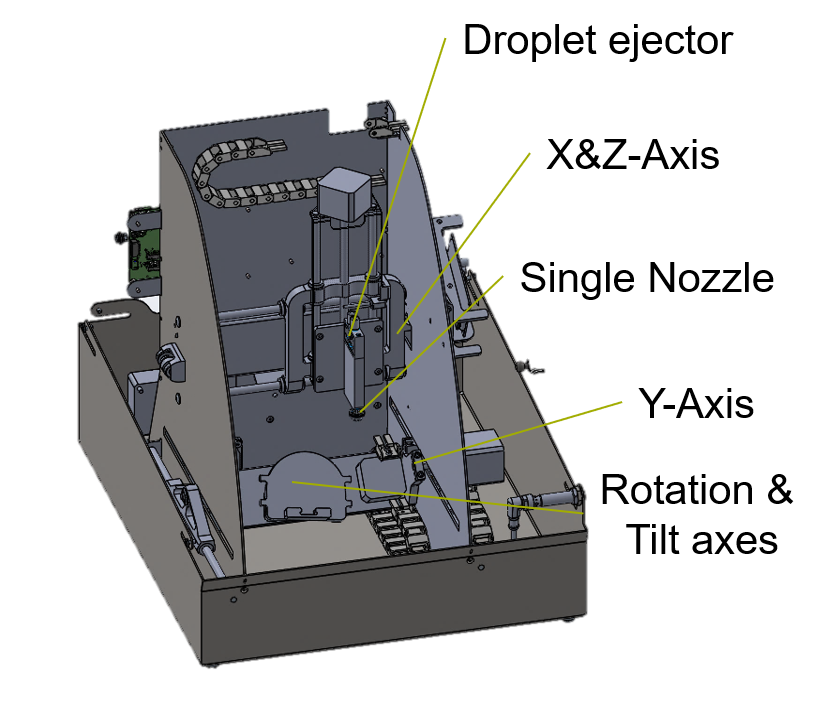
\includegraphics[width=0.7\textwidth]{grafiken/PrototypeText.png}
	\caption{5 axis printer design for dental ink (Matthias Leininger, Bredent GmbH)}
	\label{fig:Prototype}
\end{figure} 

\bigskip

\section{Material Properties}
For a dental technician it is completely trivial how viscous the ink is but for an automated printing  process the quantization of the properties is highly important. In the first experiment, the properties of the coloring agents A1, A2 and A3.5 are determined and compared to those of water. The inks have a similar density to water, but with increasing coloring agent the surface tension gets lower and the viscosity gets 3 times higher when compared to water. Also, a porosity measurement for the zirconia is conducted, which revealed a 43 percent void fraction. The raw volumetric porosity measurements are 43.09,	43.00 and 43.70. The consistency of the results is also a sign for randomly close packed zirconia powder during the manufacturing procedure. Otherwise the irregular packing would inhibit the fluid drainage and cause macro voids inside the porous material after the dissipation of the impregnating liquid, which would also lead to porosity measurements with a significantly large standard deviation. 

\bigskip

\begin{figure}[H]
	\centering
	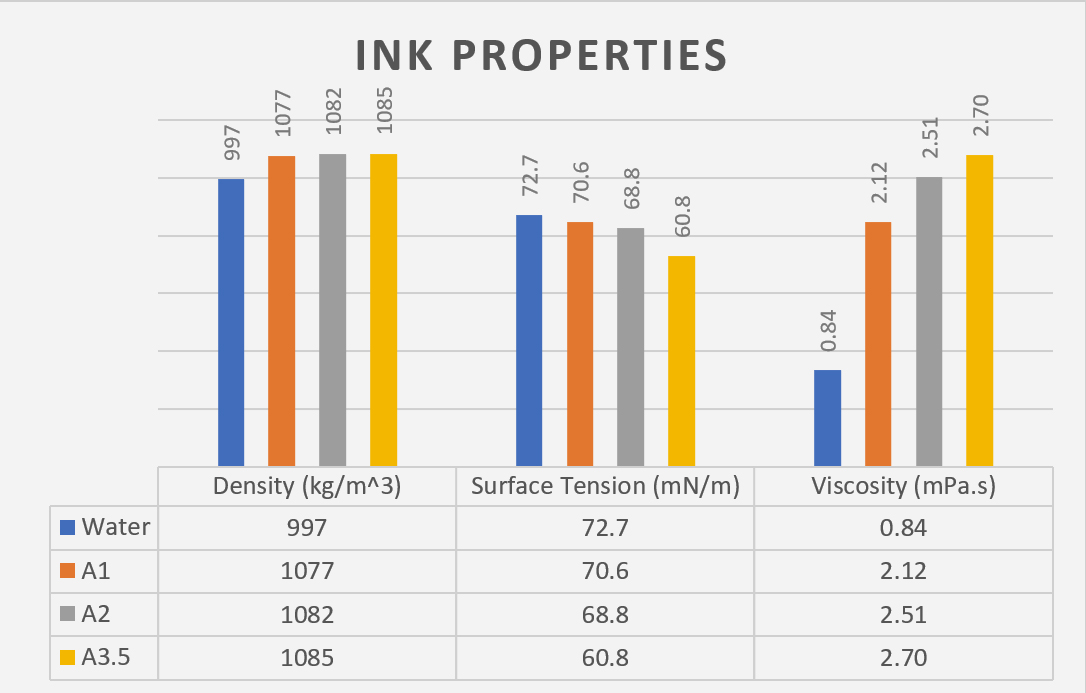
\includegraphics[width=0.8\textwidth]{grafiken/InkProps.jpg}
	\caption{Ink Properties}
	\label{fig:InkProps}
\end{figure} 

\bigskip

The most important outcome of this experiment is high values of viscosity observed for the inks, in comparison to water. This situation provides numerous advantages for the drop generation part of the process. The higher viscosity of the ink helps reduce the occurrence of the satellite drops.
\begin{comment}
 \section{Ink Concentration vs. Shade without Lateral Flow}

The dental colors appearing after the sintering process have to be assigned to specific ink concentrations. When a pattern is printed on the zirconia surface a part of the ink deployed on the target area escapes the region where t is supposed to be through lateral diffusion in the pores of the material. That is the reason one observes a spread distribution of color intensity. This can be inhibited if the whole material is printed with the same amount of ink to assure a homogeneous color intensity throughout the whole surface to obtain the theoretically achievable shades without the influence of lateral diffusions inside the material.

In order to conduct the experiment, 10 zirconia plates are prepared in a square form. The surface of the plates are imprinted with the amount of ink which is equal to the 0\%, 10\%, 20\%, 30\%, 40\%, 50\%, 60\%, 70\%, 80\%, 90\% und 100\% of the calculated porosity of the zirconia plates. The color intensities are calculated later with the results of the PSF experiment.

\end{comment}

\section{Absorption Time}
The second experiment is about the absorption time of the droplets which limits the printing time. Before the first drop is absorbed, a second drop should not land on the same spot. This would lead to accumulation of the liquid on the surface and eventually they would flow in the direction of the first drop because of the surface which is already wetted. The target accuracy of the drop deployment system would lose all of its importance. The resolution would be also sacrificed alongside the target accuracy, due to the accumulated liquid on the surface. The absorption time is formulated by Markicevic et al. as in equation \ref{eq:InfTime}.

Depending on the Eötvös rule, the surface tension of any Newtonian liquid declines with climbing temperature values. For water the formula is generated as:

\bigskip

\begin{equation}\label{eq:watergamma}
\gamma =0.07275 \cdotp(1-0.002\cdotp(T-291))
\end{equation}

\bigskip

Arrhenius-Andrade-Relation defines the viscosity of any Newtonian fluid depending on the temperature in the equation \ref{eq:viscosity}.  

\bigskip

\begin{equation}\label{eq:viscosity}
\eta =\eta_0 \cdotp exp(\frac{E_A}{R\cdotp T})
\end{equation}

\bigskip

The exponential reduction of the viscosity  versus the proportional decrease of the surface tension would be expected to result with a cumulative decrease of the absorption time with climbing temperatures.

Single drops with a volume of 100 nL are deployed on the sawn and milled surfaces. The time between the landing and complete absorption was measured 4 times for each surface structure at the temperatures 20\textdegree \space C, 30\textdegree \space C, 40\textdegree \space C, 60\textdegree \space C and 80\textdegree \space C.

\bigskip

\begin{figure}[H]
	\centering
	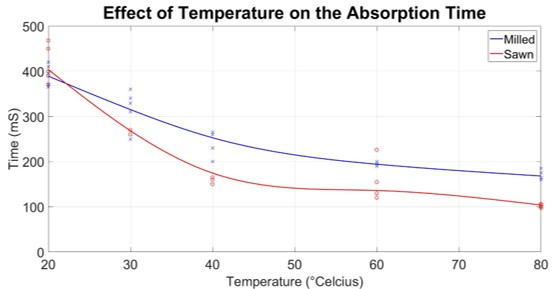
\includegraphics[width=0.8\textwidth]{grafiken/AbsorptionTime.jpg}
	\caption{Effect of heat on the absorption time}
	\label{fig:AbsorptionTime}
\end{figure} 

\bigskip

Analyzing the collected measurements, it can be concluded that a 60\textdegree \space C increase of the zirconia plate leads to about 50\% decline of the absorption time. Thus the printing time also gets reduced to half of the duration it would take under room temperature.
 
\section{Drop Size Selection}
The purpose of the third experiment is deciding for an adequate drop size. A larger drop size results in shorter print duration. However they also tend to expand the spot area more compared to the smaller drops, even though the porous material is not close to being saturated, which is a serious problem for the resolution. Depending on the drop size, the drop generation method is to be selected.
 
\bigskip
\begin{figure}[H]
	\centering
	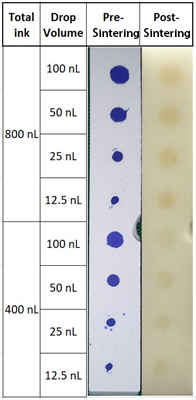
\includegraphics[width=0.36\textwidth]{grafiken/DropSize.jpg}
	\caption{Effect of the drop size on the spot area}
	\label{fig:DropSize}
\end{figure} 
\bigskip

In the figure \ref{fig:DropSize} one can see a printed zirconia specimen. Each spot on the upper half has a total ink volume of 800 nL and the ones on the bottom half 400 nL. These spots are printed using drops with volumes of 100, 50, 25 and 12.5 nL.The first image shows the spots right after printing. The second one shows the surface after furnacing.

\bigskip

\begin{figure}[H]
	\centering
	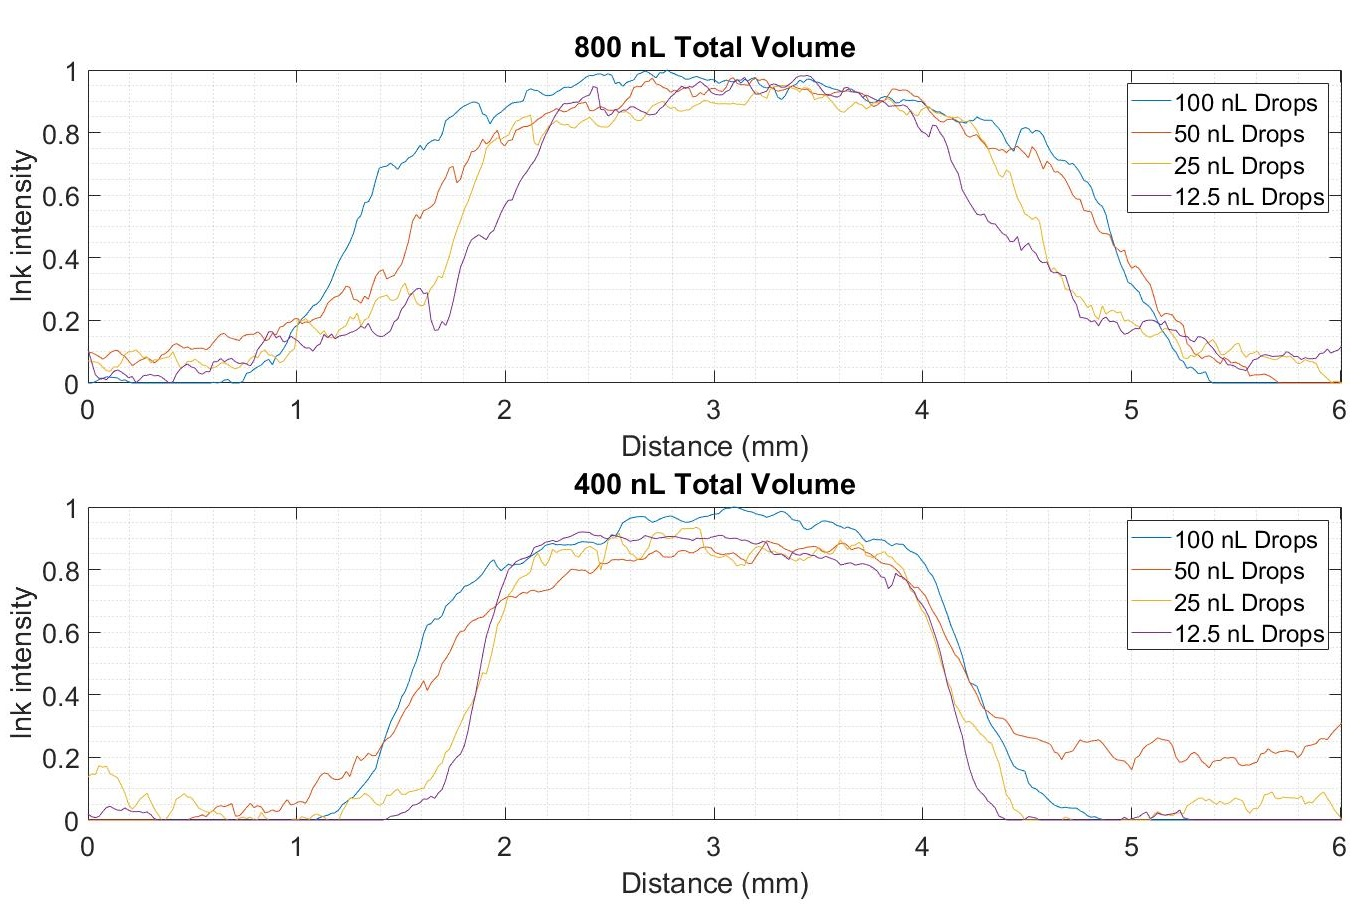
\includegraphics[width=1\textwidth]{grafiken/SpotArea.jpg}
	\caption{Comparison of the spot area results depending on the drop size}
	\label{fig:SpotArea}
\end{figure} 

\bigskip

The graphs show the ink intensity along the red lines and the spreading of the ink in lateral direction for each drop volume. 12.5 and 25 nL drops result in a similar spot diameter but the spots tend to get significantly larger with 50 and 100 nL Drops. Depending on these results 25nL can be selected as the optimum drop size for further experiments. However, considering to repeat some key procedures for the drop size of 50 nL can also be advantageous to gather further information.

\section{Proximity}

The proximity effect describes in the case of dental printing the coloring of the unprinted area between two printed areas proximate to each other. The closer the printed areas are, the saturated becomes the unprinted area in between.

If the color change of the unprinted area can be described depending on the ink concentration and distance between the printed areas, the effect of the proximity can be implemented to the model. During this experiment an exception is made and for the printing process a drop size of 12.5 nL is chosen. This is the smallest volume the printing system can generate stably, without spraying the ink in a circle or generating satellite droplets. The reason for selecting the smallest possible droplet volume is to rule out or at least minimize the lateral flow of the ink caused by the initial wetting area.  

\bigskip

\begin{figure}[H]
	\centering
	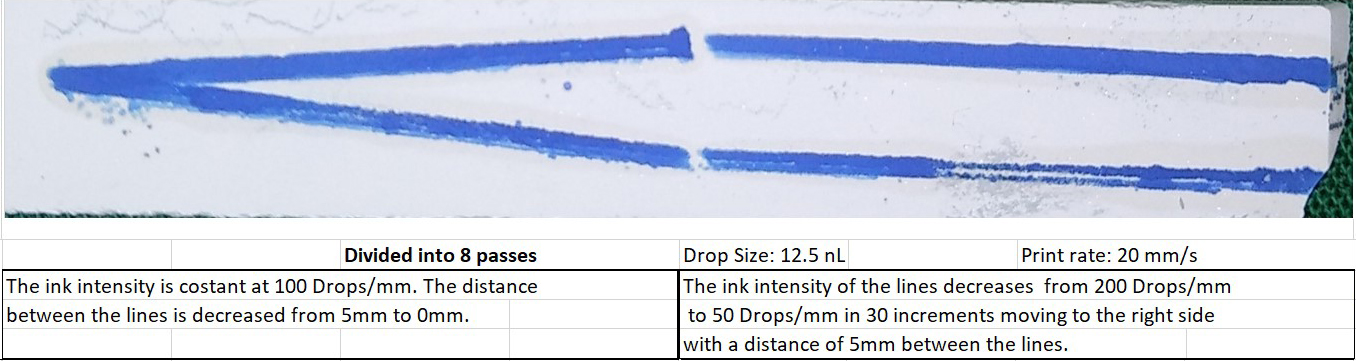
\includegraphics[width=1\textwidth]{grafiken/proximityprint.jpg}
	\caption{Printed pattern for the proximity effect}
	\label{fig:proximityprint}
\end{figure} 

\bigskip

A pattern with varying distance between two lines and another pattern with varying droplet concentration were printed on the zirconia. The blue lines mark the initially printed surface portion before the sintering process, without taking the diffusion of the ink in the material into account. The dental ink is not easily recognizable by the naked eye before the sintering process, but it can diffuse far into the zirconia. The the blue ink is added to the dental ink bottle to make the printed area recognizable. However, The blue ink cannot infiltrate the zirconia as good as the dental ink and gets filtered, gathering mostly on the initial contact area. If the Figure \ref{fig:proximityprint} is observed closely, one can recognize a slightly darker trace around the blue lines in comparison to the natural whiteness of the zirconia surface. The darker regions are infiltrated by the dental ink and seem to have a definite border. However, the sharp transition from the infiltrated to dry cannot be withhold for after the sintering process.

The pattern on the left size presents two lines starting on the same coordinates and reaching a distance of 5 mm at right end. The ink trace has a constant concentration of 1250 nl/mm. The pattern on the right side presents two lines with a constant distance of 5mm to each other. On the left end of the lines, the ink intensity is 625 nl/mm and reaches linearly 2500 nl/mm towards the right end of the pattern in 30 incremental steps.

\bigskip

\begin{figure}[H]
	\centering
	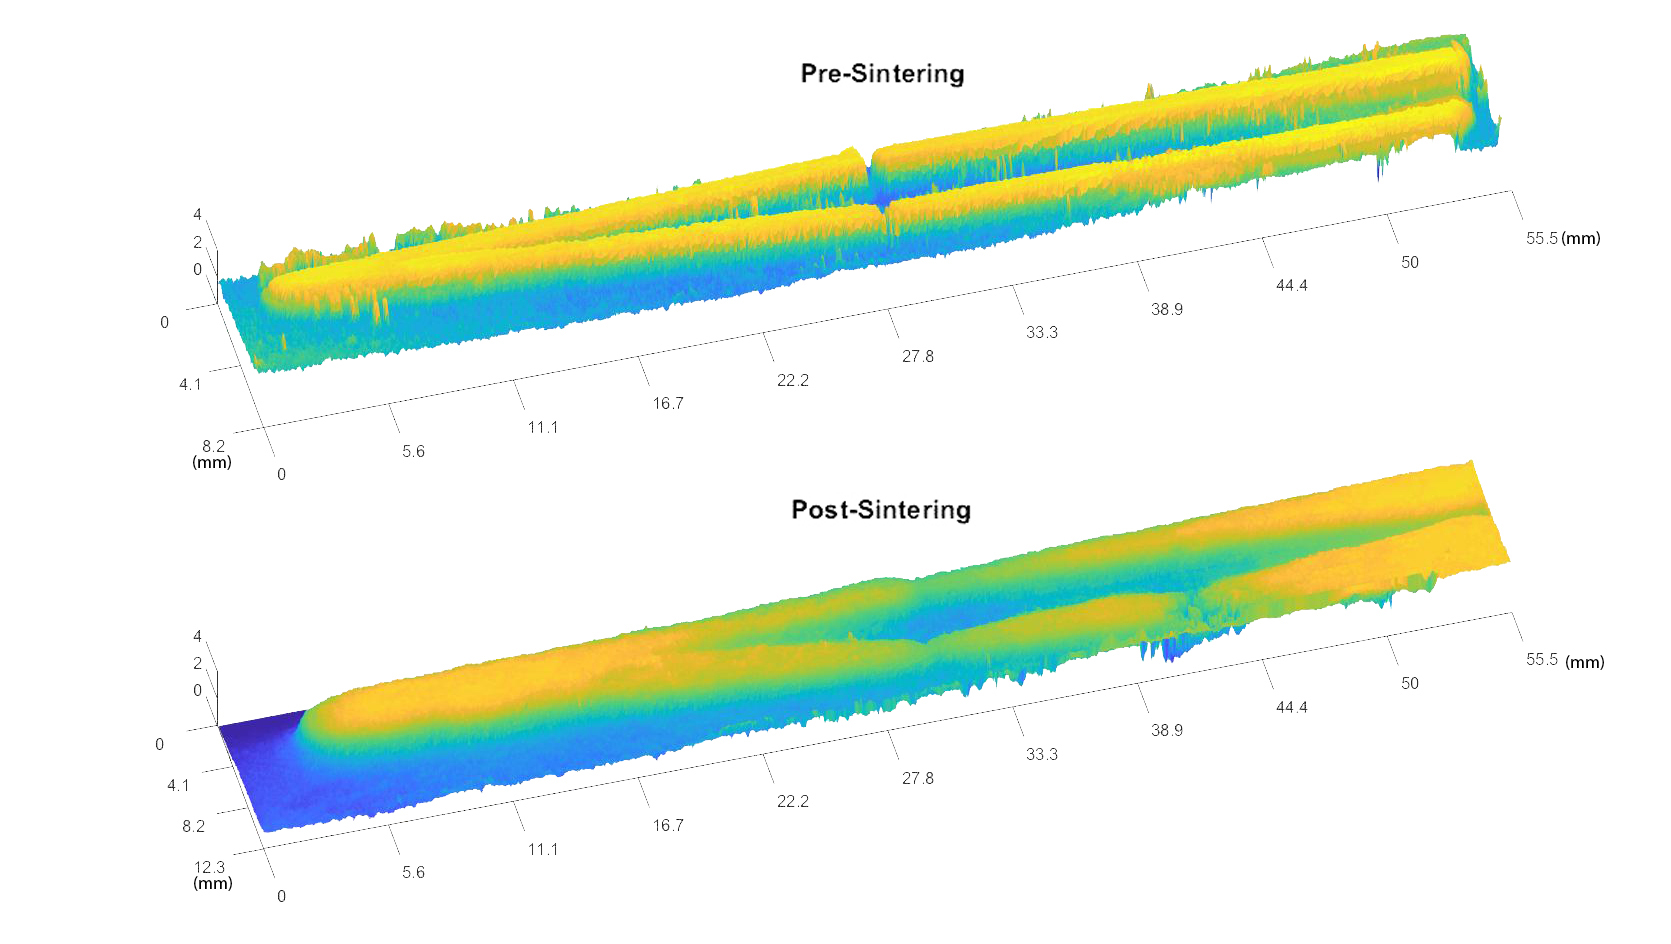
\includegraphics[width=1\textwidth]{grafiken/prepostV.jpg}
	\caption{Ink intensity analysis of the printed pattern before and after the sintering process}
	\label{fig:prepostV}
\end{figure} 

\bigskip

Observing the Figure \ref{fig:prepostV}, one can qualitatively conclude, that the proximity has a significant effect on the coloring behavior. More than a half of the pattern seems to be one thick line on the left side of the postsintering graph in contrary to the lines recognized in the presintering analysis graph. 

The second pattern with the varying ink intensity contains a flaw. The lower line is weaker in the middle because of a contamination with finger oil, which happened before the printing process. Nevertheless, the experiment was proceeded in order to observe, how seriously the printing process is affected by a slight finger oil contamination. The result shows a serious fluctuation in the acquired color which is as high as two shades. 



\bigskip

\begin{figure}[H]
	\centering
	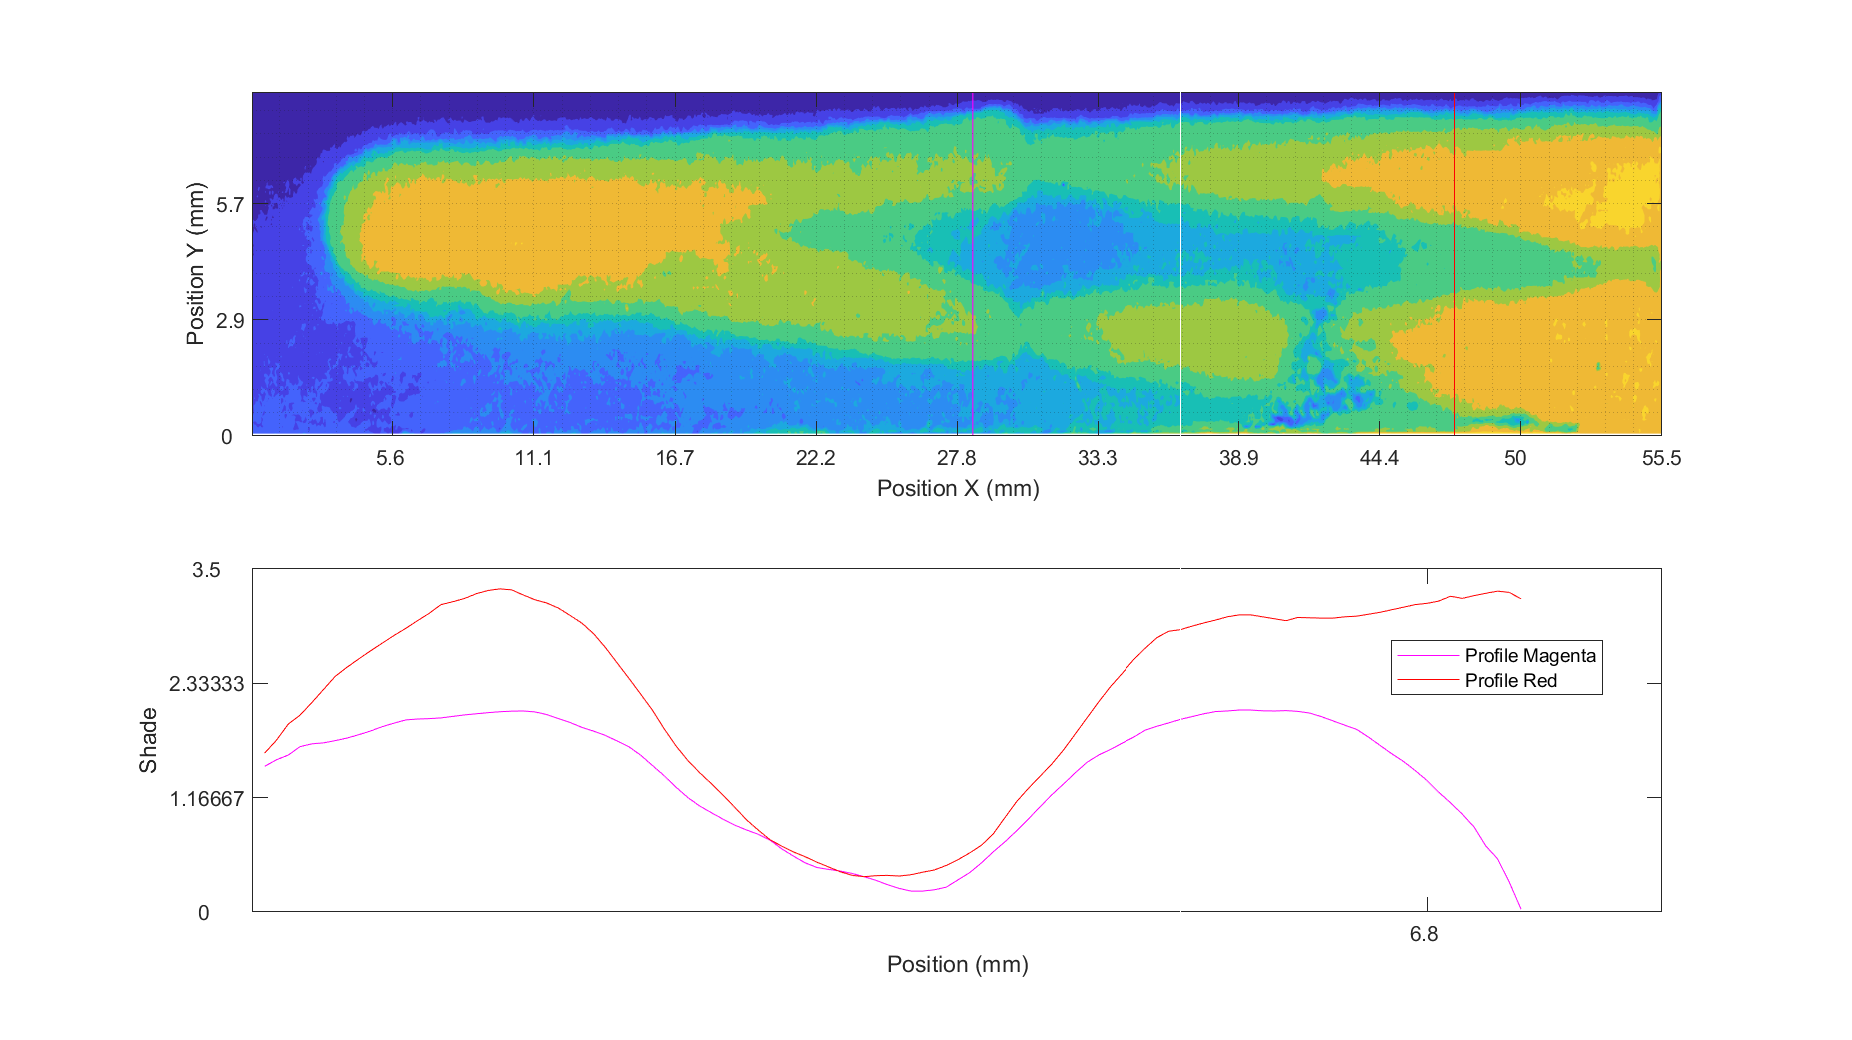
\includegraphics[width=1\textwidth]{grafiken/vmatch.eps}
	\caption{Comparison of two profiles belonging to imprints with identical parameters}
	\label{fig:vmatch}
\end{figure} 

\bigskip

The purpose of the experiment was to define the optimum trace distance for various ink intensities. The result of the first pattern is to be utilized to confirm the integrity of the results of the second pattern. The ink distribution on the line, where the distance between the two lines is 5 mm in the first pattern, magenta line in the Figure \ref{fig:vmatch}, should be the same with the ink distribution along the red line on the second pattern in the Figure \ref{fig:vmatch} where the printing ink intensity is 1250 nl/mm. If the results would comply with each other, the optimum trace distance for any ink intensity could be calculated. However, the effect of the lateral diffusion was underestimated at time of planning the concept, which resulted with a divergent result that can be observed in the lower graph in the Figure	\ref{fig:vmatch}. The ink diffusing from the higher intensity regions on the right side increase the intensity of the regions on the left side, so that the color intensity distributed over the red line does not belong to the printing intensity of 1250 nL/mm.

\bigskip

\begin{figure}[H]
	\centering
	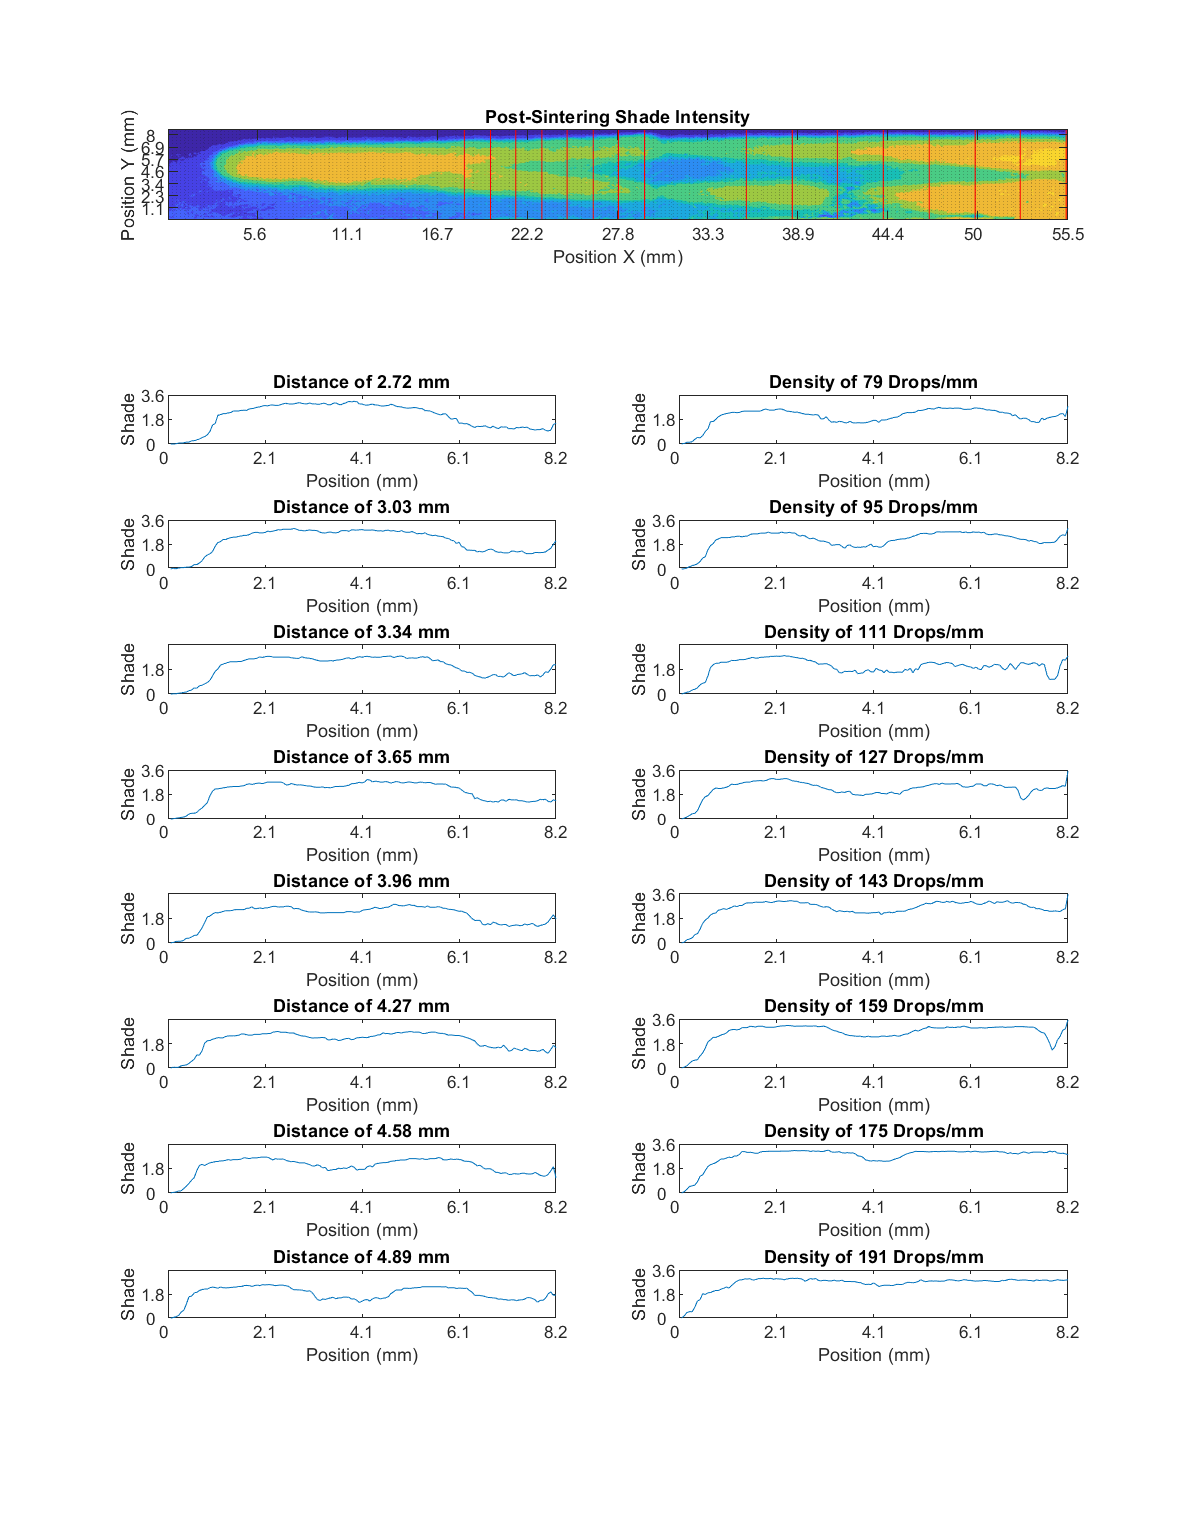
\includegraphics[width=1\textwidth]{grafiken/vProfile.eps}
	\caption{Profiles of color intensity depending on the distance on the left and depending on the ink amount on the right}
	\label{fig:vProfile}
\end{figure} 

\bigskip

The plots to analyze the ink distribution are presented separately in two columns in the Figure \ref{fig:vProfile}. The column on the left side presents 8 equidistant positions on the varying distance pattern which are marked with eight red vertical lines and the right column contains the cross section of the pattern on the right side with varying ink intensities. The pattern on the left shows that a necking appears already with a distance of 3 mm when the printing intensity is equal to 1250 nl/mm. In other words, printing with a trace distance higher than 3 mm result with an unwanted brighter stripe in the middle of printing traces. Whereas, a trace distance lower than 3mm cannot result with a more saturated color but a higher diffusion range or a thicker single line. 

The data acquired from the first pattern was planned to be matched with the data from the section with the ink intensity of 1250 nl/mm on the second pattern but the extreme irregularity levels of diffusion in the x direction make the data acquired from the second pattern quite useless. Not to mention a direct match and acquisition approach, it is even not possible to calibrate the data on the second pattern to conduct trace distance calculations, because of the nonlinear lateral ink distribution inside the material along the second pattern. 



\section{Printing Angle}
The dental crowns do not always present convex features. The chewing surface can rarely possess even some undercut geometries. In such cases, it is not possible for a droplet to land on the zirconia surface vertically and for some known areas, the printing process has to be conducted on skew surfaces. 

If the lateral momentum of the droplets are high enough at the moment of the impact on the surface, the printed pattern can look like it has a motion blur effect. It is also possible that the resolution gets lower because of the lateral flow of the drops on the surface. There has to be some critical angle at which such disadvantages become inevitably  significant. The maximum milling angle used for the dental crowns is declared by Bredent GmbH to be 30\textdegree \space. So, an experiment to test the effects of printing on a skew surface up to an angle of 45\textdegree \space is supposed to be comprehensive enough.

	\bigskip

	\begin{figure}[H]
		\centering
		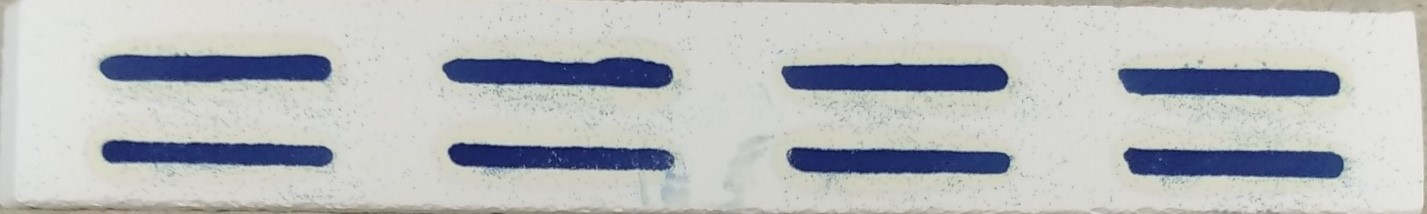
\includegraphics[width=1\textwidth]{grafiken/angleprint.jpg}
		\caption{Comparison of the spot area results depending on the drop size}
		\label{fig:angleprint}
	\end{figure} 

	\bigskip

In order to test the effect of printing on a skew surface two parallel lines are printed on the surface which have a distance of 4 mm. This process is repeated 4 times, while the zirconia specimen was standing at angles 0\textdegree \space, 15\textdegree \space, 30\textdegree \space and 45\textdegree \space. The printed sample can be seen in the Figure \ref{fig:angleprint}. The highest possible printing angle that could be required is defined by the dental technologists from the Bredent GmbH to be 30\textdegree \space because of the traditional parameters of the milling process. The maximum milling angle for the inner features of the crown is realized by a CNC with a machine tool angle of 30\textdegree \space to the crown axis. So the extension of the experiments up to a printing angle of 45\textdegree \space is slightly off the limits but necessary to be on the safe side.

The lines were generated using 25 nL droplets with a drop density of 50 drops per mm. The thickness of the lines are measured as 2.2 $\pm$ 0.1 mm. The measurements of the thicknesses as 2.2 mm on the specimen belong to the blue lines, which present the contact area on the zirconia with the ink. 2.2 mm is not the thickness of the lines after the sintering process. The consistency of the thicknesses at all angles is enough for the observer to draw the conclusion that the printing angles up to 45\textdegree \space do not cause any significant change in the printed pattern. If the wetted surface on the zirconia is the same for all of the printing angles, the possibility of observing different line properties after the sintering process is quite close to zero.

\section{Singular Spot Characteristics}

Since the efforts to determine the characteristics via continuous lines did not provide conclusive results because of the ink diffusion inside the porous material, discontinuous, isolated imprints are required as a further experiment. 8 Spots are to be printed with an equidistant placement. The distances between the spots are 8 mm which is beyond the diffusion range of the relative ink amounts. 25 nL drops and 50 nL drops are deployed on two different specimen to observe the effect of the droplet size depending on the total ink volume. 

The drops are expected to have a high color intensity in the middle. That middle point is going to be the center of the Gaussian distribution. The points with an equal distance from the middle are supposed to present a point symmetrically identical color intensity.

\bigskip

\begin{figure}[H]
	\centering
	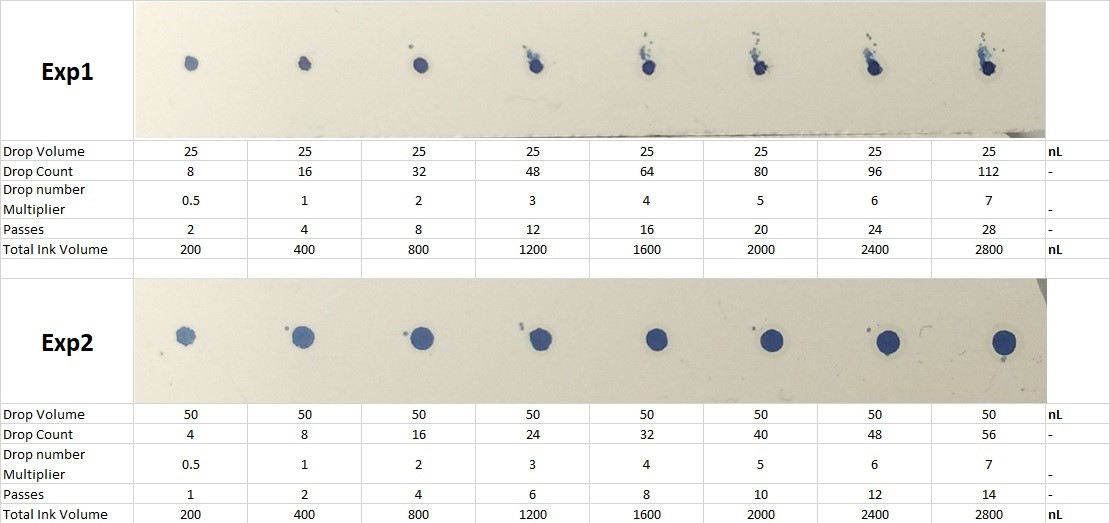
\includegraphics[width=1\textwidth]{grafiken/psfprint.jpg}
	\caption{Comparison of the spot areas depending on the drop size and total ink amount}
	\label{fig:psfprint}
\end{figure} 

\bigskip

The Figure \ref{fig:psfprint} presents both of the printed zirconia plates before the sintering process combined with additional tables to sort the properties of each printed spot in a well defined manner. 

In order to inspect the Gaussian distributions of the ink intensities in cases of different total ink amounts and different drop sizes 8 spots are printed using drops with volumes of 25 nL and 50 nL. The total ink volumes for the spots on each plate are identical and equal to 200 nL, 400 nL, 800 nL, 1200 nL, 1600 nL, 2000 nL, 2400 nL and 2800 nL.
\begin{comment}
The results of this experiment are necessary for the reverse calculation of the required ink amount. Depending on the calculations a map can be generated for the amount of drops and target positions to deploy these drop, in order to acquire a desired shade distribution as an outcome.  
\end{comment}
The lack of a color sampling device for shade measurement, channeled the color determination process to a software solution. The images captured with a standard camera are edited via MATLAB to acquire data about the color intensities. After the sintering process, the plates were laid on a homogeneous light source with a constant output level of 570 nits. The color distribution observed on the front side of the plates was captured using a high resolution camera. The captured image is processed utilizing the image processing toolbox of MATLAB. What important was, that the colors were not drifted out of scale during the editing processes which would make all of the results useless for further calculations. In order to increase the global contrast, histogram equalization is conducted. The working principle of the histogram equalization process is similar to apllication of a band pass filter after an analysis is made with the Fourier transform. The intensities of different wavelengths in the image are analyzed. The interesting part of the wavelength spectrum is cropped and distributed over the whole visible spectrum conducting a linear scaling. This process makes it easier to distinguish between the slightest color changes. Then the image is converted from an RGB image to a gray scale one, since the intensities of the 3 colors are not individually relevant to the purpose of the experiment. 

After this point, the darkness of each pixel presents its color intensity. Since the image contains a region which is printed beyond the maximum saturation level, a small pixel region with the highest intensity can be used for calibrations purposes as a dental shade of A3.5. The calibration shade is A3.5, because at the time of the development processes A3.5 is the most saturated shade provided by the research partner. Calibrating the other end of the spectrum for the lowest intensity is not such a straightforward calculation. Each line of the image actually has a slight different illumination because of the irregularities on the edges of the zirconia plate or even some defects on the  plate like curved surfaces due to sintering process or broken regions.

One example to such defects can be observed in the Figure \ref{fig:drops25} on the false colored intensity image positioned on the left side. Just below the second spot from the top are lots of pixels contaminated with intensity noise. The reason for that is a crack in the plate, along the x-axis, at the position y=49 mm. Since the wall of the plate at breaking line is not parallel to the XZ-Plane and does not have planar surface, the light guided into the material is not homogeneous either. 

The calibration of the lowest intensity is made because of the mentioned reason separately for each line of the zirconia image. At each level it is known that the regions close to the edges of the zirconia plate contain no coloring agent. Edges of the plate are also illuminated with different intensities in comparison to the continuous regions in the middle. Thus, the minimum intensity value is obtained cutting out the regions close to the material border and taking  the minimum intensity as a reference point for the shade A0.
\bigskip

\begin{figure}[H]
	\centering
	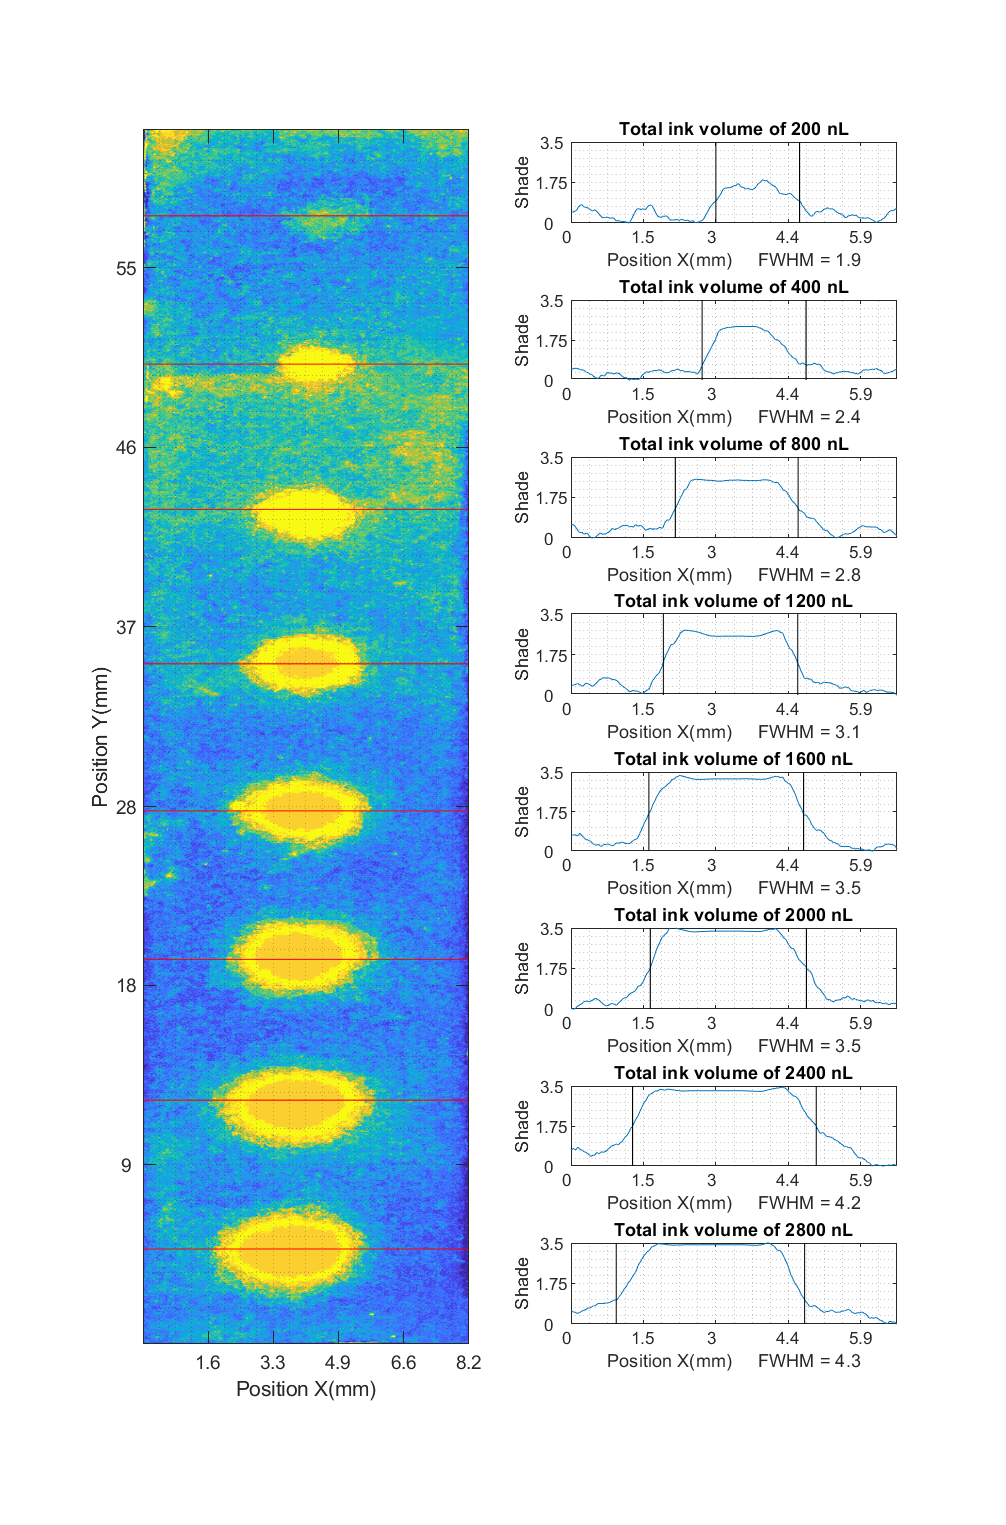
\includegraphics[width=0.8\textwidth]{grafiken/drops25.eps}
	\caption{False color representation and shade spreading analysis of the spots after sintering (printed with 25 nL drops)}
	\label{fig:drops25}
\end{figure} 

\bigskip 

Due to the nonlinear printing characteristics of the porous zirconia medium, a proportional intensity change cannot be observed along increasing total ink amounts. As a reminder, it should be said that the printing process is realized using an ink with a calibrated shade of A3.5. This means if the zirconia plate is sunk into the ink completely and hold in the ink for at least 10 seconds so that there is relatively no air left in the porous medium, the end color shade of the zirconia would be an A3.5. This global void filling condition can also be fulfilled locally with the inevitable occurrence of some lateral diffusion. 

There are two parameters one should pay attention to on the plots positioned on the right side of the Figure \ref{fig:drops25}. One of them is the shade, the other one is the Full Width Half Maximum (FWHM) measurement of the spots. Each plot belongs to the line on the false colored image, on the same height with the plot. The applied amount of ink on the first spot is 200 nL. Even though the plot has a global maximum around A1.75, the results are not trustworthy, because of the noise level on the line. The areas close to the edges reach easily 50\% of the global maximum which is a sign of low signal to noise ratio and is caused by extremely low amount of the applied ink. 

The spots with total ink amounts of 1600 nL and 2000 nL present the same FWHM value which is equal to 3.5 mm. The 1600 nL total ink amount brings the graph just below the shade A3.5, but the total ink amount 2000 nL reaches the shade A3.5 with a constant level plateau. This means 2000 nL is the critical value for full saturation under lateral diffusion conditions. A higher amount of ink causes only a proportionally larger FWHM. For 25nL Drops it can be said that different shades can be obtained using an ink with the shade A4.0 and a brightener with a total amount of 2000 nL on each spot.

\bigskip

\begin{figure}[H]
	\centering
	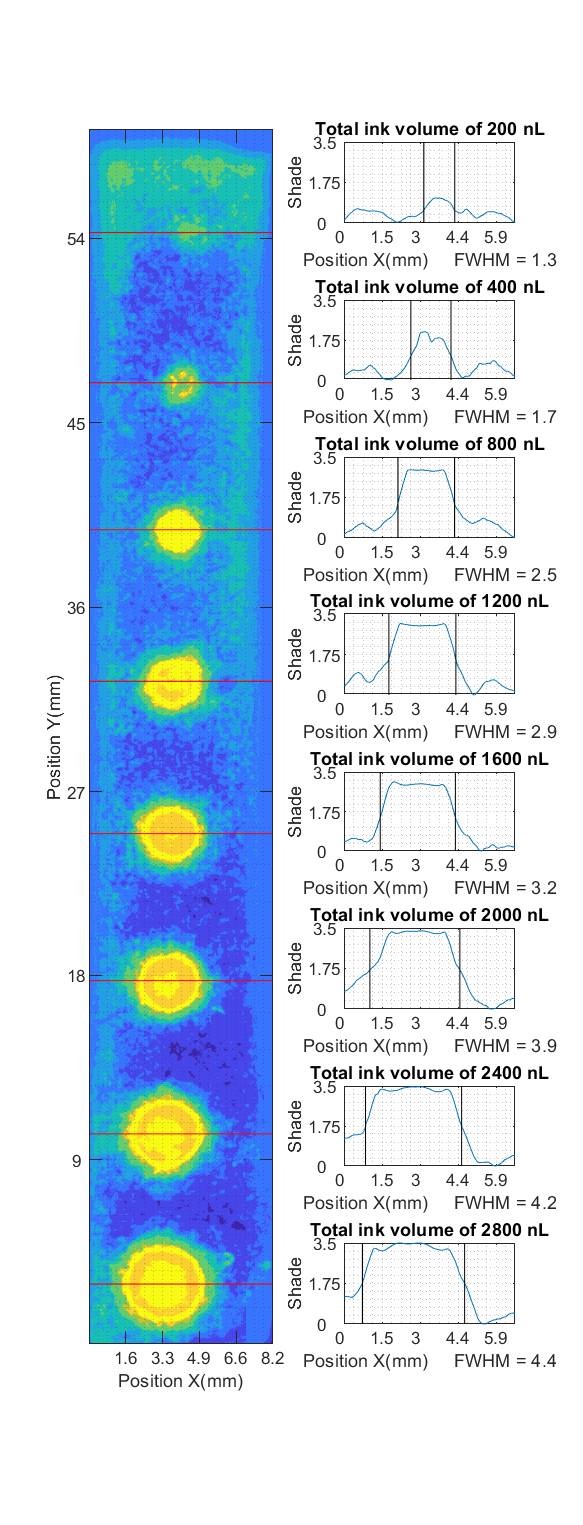
\includegraphics[width=0.8\textwidth]{grafiken/drops50.eps}
	\caption{False color representation and shade spreading analysis of the spots after sintering (printed with 50 nL drops)}
	\label{fig:drops50}
\end{figure} 

\bigskip 
 The same experiment is repeated for the drop size of 50 nL with the half amount of drops to achieve the same total ink amount. The only practical difference between the experiments is the diameter of the first contact circle. When the first wetting area is larger the ink tries to impregnate the zirconia through a larger area which means that the lateral diffusion is supposed to happen easier and the FWHM diameters are to be slightly larger than the ones belonging to the 25 nL droplets depending on the Equation \ref{eq:SpreadingDia} . It is hard to conduct a comparative evaluation for the first four spots from the top because of the high noise generated by the crack in the first specimen. 
 
 The spot created with 1600 nL ink has a lower shade level in comparison because of the higher diffusion distance of the ink caused by the larger initial contact. If the initial contact area is larger, the ink is transfered beneath this larger area into the zirconia material. After the impregnation the diffusion can happen beginning from a comparatively larger area which means that the ink can reach further away, but with less intensity. Since the ink is distributed more to the outer circles, the intensity of the 1600 nL spot is lower for 50 nL drops in comparison to 25 nL ones.
  
 The total ink amount of 2000 nL is again enough for the full saturation of the pores. The predefined shade of A3.5 is reached with a large plateau as a sign for the saturated spot imprint with an FWHM of 3.9 mm. The FWHM values for the ink amounts 2000 nL, 2400nL and 2800 nL in the first experiment were, as it can be seen in Figure \ref{fig:drops25}, 3.5 mm, 4.2 mm and 4.4 mm. Those values are 3.9 mm, 4.2 mm and 4.4 mm in the second experiment. The fact that the last two diameters are exactly the same for both of the drop sizes shows that an amount of total ink this high is significantly over the saturation limit of the spot area. 
 
 There is another important result one can conclude out of these two samples. If the printing process was done with a color shade of A4.0 and the target shade was A4.0 ,the whole void proportion of the material would have to be filled with the ink for the shade A4.0. Whether the drops have a volume of 25 nL or 50 nL doesn't change the fact that the material has to be filled up regionally and this will cause inevitable  lateral diffusions. Thus it is not quite likely to obtain A4.0 spots as tiny as A1.0 spots using an ink with a shade of A4.0. Because in the upper plots of the Figures \ref{fig:drops25} and \ref{fig:drops50}it can be observed that the spots have shades below A1.75 and the FWHM values are less than or equal to the half of the saturated A4.0 generating spot diameters.
